\chapter{Electric characterization}
\label{ch:electric}
\section{Electric scheme and description}
In this chapter is discussed the development of Plasma Coagulation Controller eletcric scheme and its characterization. Circuit design, as the entire model design, is highly influenced by needs of flexibility and mobility of the source for wound treatment. To produce plasma as DBD, in air, with helium or argon as ignition gasses, it is necessary to apply high electric fields in little space. Manwhile, to make possible easy medical application the source head (where there si plasma output) must be compact, with particular attention to electric safety measuraments.
It is common to produce electric fields with fast voltage pulses for various uses, including jet or DBD plasma production (\cite{Upadhyay:hvpulse}, \cite{Jarrige:plumecharacteristics}, \cite{Darny:jetplume})), the scheme used in this study outputs a voltage pulse with an amplitude from $\SI{1}{\kilo\volt}$ to $\SI{10}{\kilo\volt}$ and pulses frequencies from $\SI{5}{\kilo\hertz}$ to $\SI{60}{\kilo\hertz}$.

A rappresentation of power and signal lines is in figure \ref{fig:electricline}. The circuit is divided mainly in two parts %as described in chapter \ref{ch:source}
: the controller, with alimentation and settings controls, and the head, where the discharge happens and plasma is emitted.
\begin{figure}
 \centering
 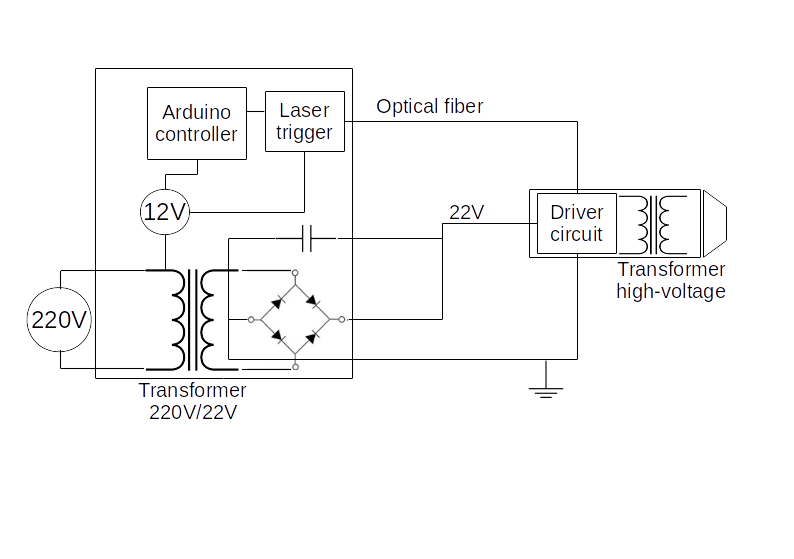
\includegraphics[width=0.8\textwidth]{Images/Electric/Linea_elettrica.png}
 \caption{Scheme of the general electric line to produce high voltage, the controller on the left and the head on the right.}
 \label{fig:electricline}
\end{figure}

Lines divides in:
\begin{itemize}
 \item \textbf{Alimentation} : the $\SI{220}{\volt}$ DC power line goes in a transformer that gives a reduced tension to the head, $\SI{22}{\volt}$ in the figure, passing through a diode bridge. This tension aliments the Driver Circuit on the head.
 \item \textbf{Arduino and trigger} : the power line is reduced to $\SI{12}{\volt}$ necessaries to aliment an Arduino controller and a laser. From an Arduino analogical output a PWM wave goes to the laser trigger, it transmits information on the wave, frequency and duration, with an optical fiber that ends with a photodiode installed on the driver circuit. Wave frequency is setted by the Arduino, wave duration is setted giving the opening time of the MOSFET that passes the signal to be amplified and sent to the head's transformer. With this setup the high-voltage line is entirely decopuled from the controller, so there are not problems of signal reflection on the power line or the Arduino.
 \item \textbf{Head} : the Driver Circuit receives a power line and an optical trigger that defines frequency and duration of the voltage pulse. When the trigger gives the start signal, the transformer on the head receives on primary circuit a voltage of hundreds $\si{\volt}$ and outputs from secondary circuit a voltage of thousends $\si{\volt}$. Connected to the output there is the electrode inside a capillary tube of dielectric material.
\end{itemize}

To understand signal propagation is presented a simulation in figure \ref{fig:signals}, obtained with a simplified scheme with Spice. As shown, once the PWM trigger starts, tension on the primary goes from alimentation value to $0$, when the PWM signal ends (after $\SI{6}{\micro\second}$, it has a pulse with amplitude of $\SI{150}{\volt}$ (width of $\SI{1.2}{\micro\second}$) and a pulse of $\SI{-5000}{\volt}$ at the output of secondary circuit. A longer PWM implies a longer charging time, so an higher pulse. Ultimately, amplitude of the pulse is proportional to the width of the PWM signal and to know working conditions of the source it is necessary to study relation between opening time and amplitude output on the actual circuit.

\begin{figure}
 \centering
 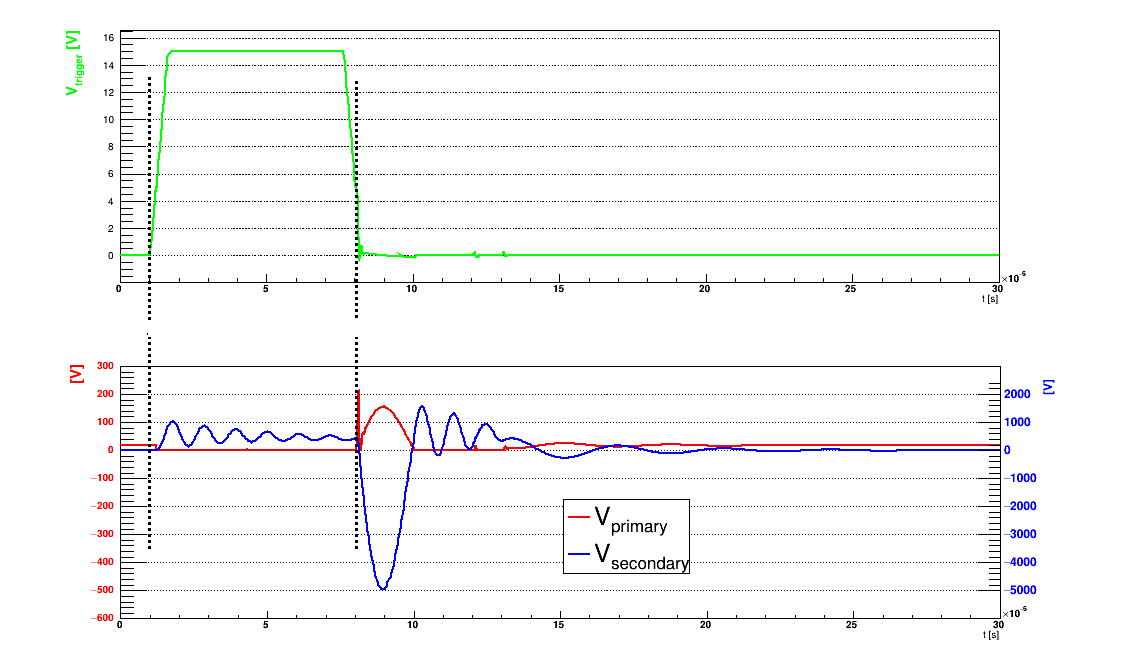
\includegraphics[width=0.8\textwidth]{Images/Electric/segnali.png}
 \caption{Scheme of signal propagation. Up, in green, there is the optical trigger, down, in red, the voltage of primary circuit in the head with axis on the left, in blue, the voltage of secondary circuit with axis on right.}
 \label{fig:signals}
\end{figure}

During this thesis study were built two sources, with two controllers and heads, the first one will be called source A, the second one source B. From an electrical perspective the two models are almost identical, the second one comes with a low-pass filter on the driver circuit (to diminish high frequencies noise) and higher amplitude capabilities thanks to a different turns ratio in head's transformer.
The characterization of electric features is made measuring output tension and current with different settings.

\section{Output characterization}
Plasma ignition and discharge features are regolated by electric field generated in the circuit head and power deposition to flowing gas, so the parameters involved are pulse amplitude and frequency arriving on the electrode, settable in the circuit. Medical application of plasma requires low current intensity, in this study it's measured current intensity flowing on a copper sheet targeted by the plasma plume at a certain distance. Ultimately the different parameters for the measures are: $\Delta t$, opening time of the trigger that defines amplitude of the pulses, and $f$, frequency of the pulses. 

Voltage signals are taken with an high-voltage probe \emph{Tektronix P6015A}, attenuation $\times 1000$, current signal with a \emph{Tektronix CT2} probe that gives a $\SI{1}{\milli\volt}$ for a current of $\SI{1}{\milli\ampere}$. All signals are measured with a \emph{Yokogawa DL9040} oscilloscope, from which is saved the waveform of voltage and current.

Measures are taken without gas flowing, to see clean output voltage of the circuit, and with an helium flow of $\SI{2}{\liter/\minute}$, to measure the actual output in presence of plasma, with different amplitude and frequencies. It's also measured an effective current intensity, i.e. a mean value in a time period, to evaluate plasma application's effects on biological tissues.

Every lenght measure is done with a decimal caliper, it's taken an uncertainity of $\SI{0.1}{\milli\meter}$.

\subsection{Measures without gas}
It's used the hv probe to pick tension's differences between secondary circuit ouput and ground.
Once a work frequency, $f$, is set, we take voltage wave shape for different values of opening time of the circuit, $\Delta t$, in the selectable range.
To assure that a voltage pulse ends before another starts, this range is different for different frequencies: higher work frequencies means more pulses in a given time, taking into consideration pulse oscillations, the range of possible $\Delta t$ is smaller at higher frequencies.
A typical measure is shown in figure \ref{fig:tensionpeak}.
\begin{figure}
 \centering
 \subfloat[Three pulses]{
    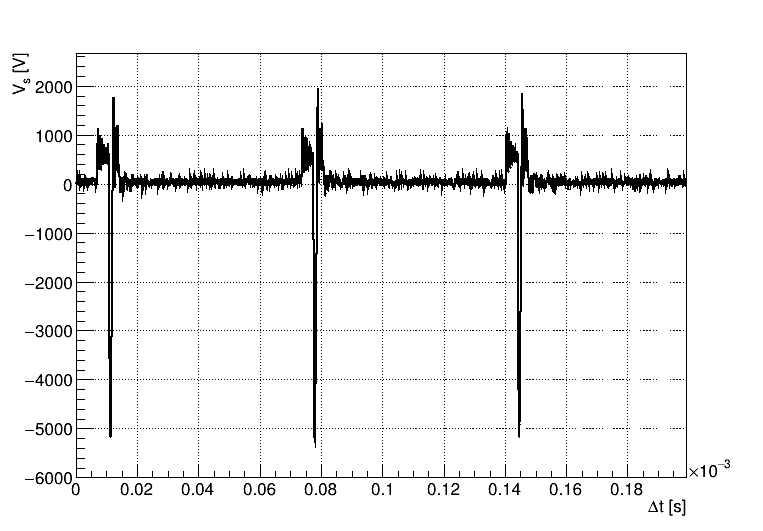
\includegraphics[width=0.40\textwidth]{Images/Electric/estrepicchi.png}
 }
 \hfill
 \subfloat[Zoom on one pulse]{
    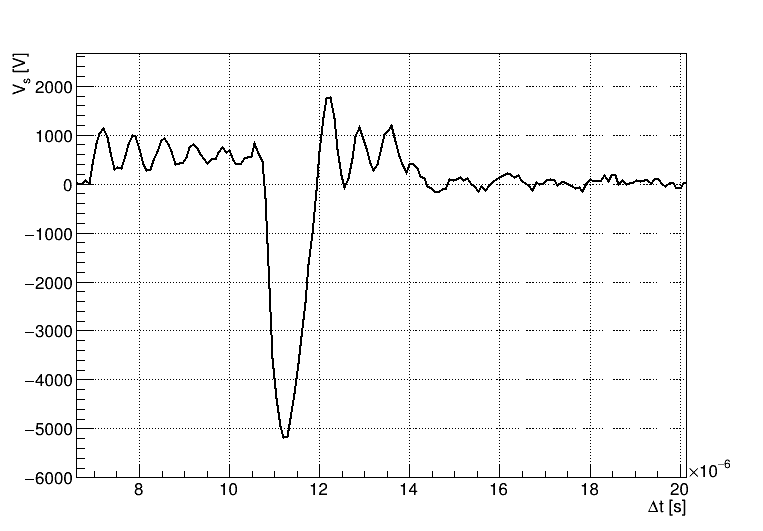
\includegraphics[width=0.40\textwidth]{Images/Electric/zoom1pk.png}
 }
 \caption{Example pulses with source B for $f = \SI{10}{\kilo\hertz}$ and $\Delta t = \SI{2}{\micro\second}$}
 \label{fig:tensionpeak}
\end{figure}

The main pourpous of the measures is to study proportionality between amplitude of the peak and opening time, for different frequencies. Those signals are analyzed evaluating their Fourier Transform (using ROOT C++ libraries \cite{ROOT:fft}) and reconstructing the signal without higher frequencies, to exclude noise fluctuations. The reconstructed peak is an asymmetric function in time as in figure \ref{fig:landau}, it's possible to interpolate it with a Landau function \cite{ROOT:landau} and obtain peak value and position.
The error from the fit function is added quadratically to the error given by the cut of high Fourier frequencies, evaluated as the square root of the mean square difference between reconstructed and original signal for every point included in fit range.
\begin{figure}
\centering
 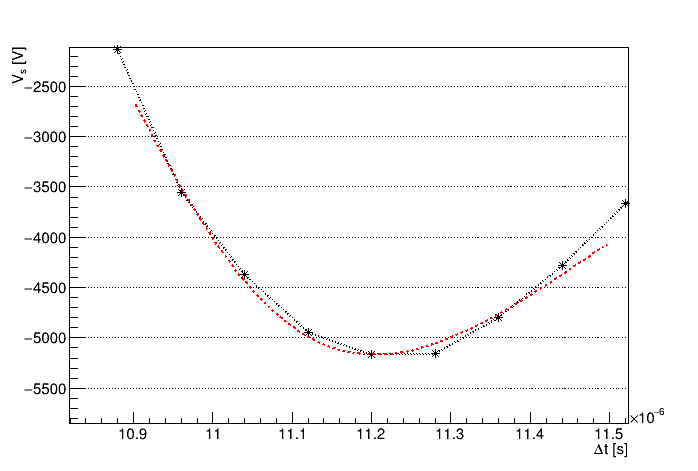
\includegraphics[width=0.6\textwidth]{Images/Electric/esfit_f10_t2.png}
 \caption{Example fit with source B for $f = \SI{10}{\kilo\hertz}$ and $\Delta t = \SI{2}{\micro\second}$}
 \label{fig:landau}
\end{figure}


Results are shown in figure \ref{fig:nogas} for the two sources.
In source A we can see a linear behavior for $4 \le \Delta t \le \SI{16}{\micro\second}$, with tensions from $\num{2.02(1)}$ to $\SI{9.25(5)}{\kilo\volt}$; for greater $\Delta t$ data loses linearity. The upper limit on chosen $\Delta t$ is given by the need of a minimum time interval between two pulses.
Also in source B we can see a linear behavior, but tension values are larger, for $1 \le \Delta t \le \SI{8}{\micro\second}$ tension goes from $\num{3.66(6)}$ to $\SI{11.76(22)}{\kilo\volt}$. With this source the upper limit for $\Delta t$ is chosen observing voltage output: measures are taken only for tensions needed to have plasma in a DBD regimen, higher opening times would only stress more circuit components.
Both sources have near the same output for different frequencies, to confirm it datas are fitted with a linear function in the range $0-\SI{16}{\micro\second}$ for source A and range $0-\SI{8}{\micro\second}$ for source B. Evalueted parameters are compared, as shown in figure \ref{fig:linnogas}. The values are displaced with random distances from the mean value, so it can be concluded that the behavior is not defined by the frequency.
\begin{figure}
 \centering
 \subfloat[Source A]{
    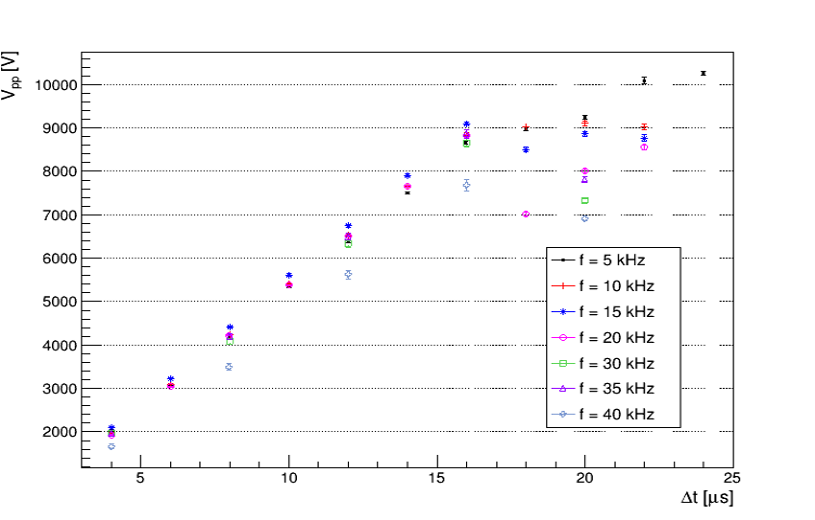
\includegraphics[width=0.6\textwidth]{Images/Electric/Vpp_nogas_A.png}
 }
 
 \subfloat[Source B]{
    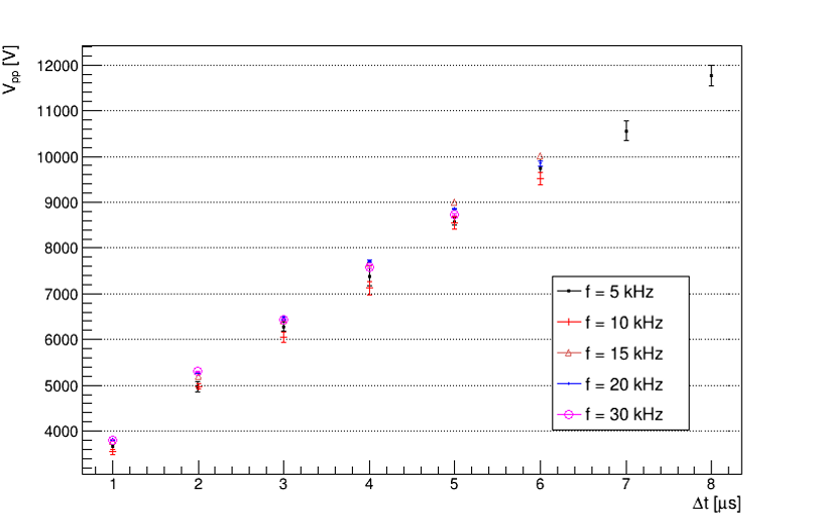
\includegraphics[width=0.6\textwidth]{Images/Electric/Vpp_nogas_B.png}
 }
 \caption{Absolute peak's value of secondary circuit in function of $\Delta t$ at different $f$, for both sources.}
 \label{fig:nogas}
\end{figure}

\begin{figure}
 \centering
 \subfloat[Source A]{
    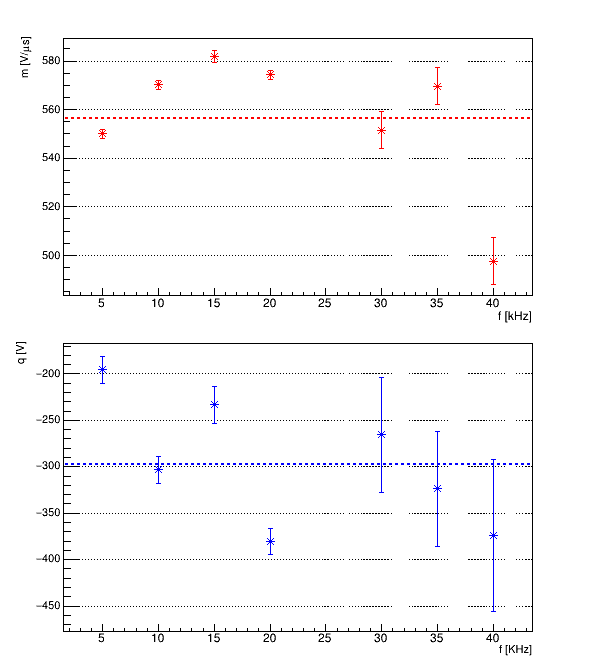
\includegraphics[width=0.4\textwidth]{Images/Electric/mq_nogas_A.png}
 }
 \subfloat[Source B]{
    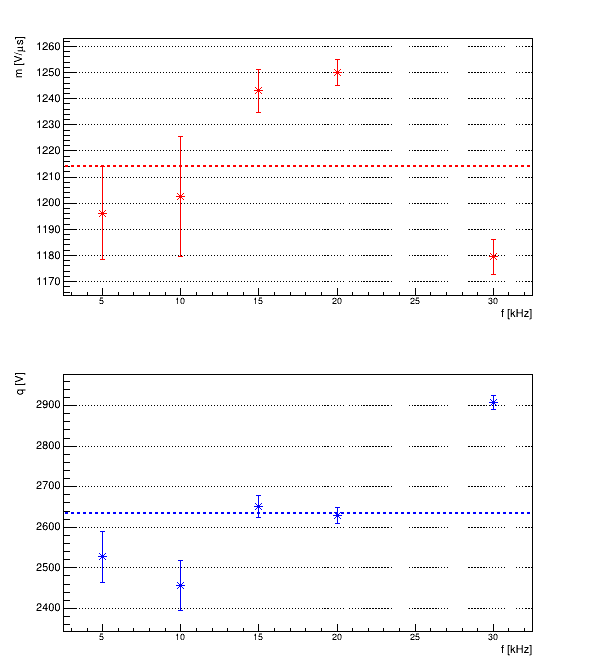
\includegraphics[width=0.4\textwidth]{Images/Electric/mq_nogas_B.png}
 }
 \caption{Voltage peaks are fitted with a linear function $V_{peak} = m \Delta t + q$, in figure we see fit parameters at different frequencies for both sources, in dashes the mean value.}
 \label{fig:linnogas}
\end{figure}


\subsection{Measures with gas}
Introduction of an helium flow at the end of the head will produce plasma ignition, tension will be different, and it will be possible to measure current intensity carried by plasma. To assure safety of plasma application, that cells aren't damaged by plasma, it must be avoided a large current intensity and arc formation. Studies of conditions for DBD discharges and arc transitions (\cite{kogelschatz:jpa-00255561}, \cite{TOMAI2006409}, \cite{PhysRev.34.876}) suggests that for fast pulses it's safe to have current intensity $< \SI{10}{\milli\ampere}$.

Current intensity is measured using a copper sheet with dimensions $\SI{10}{\milli\meter} \times \SI{10}{\milli\meter} \times \SI{1}{\milli\meter}$. Plasma plume impacts on the sheet, the current probe is connected to it and sends a voltage signal to the oscilloscope, with cable shielding to lessen interferences.
Current intensity and target distance relation is studied in\cite{unipd:ceciliaDBD}, in this study the distance between target and electrode is chosen around typical value for treatments permitted by head's sources geometry: $\SI{10}{\milli\meter}$ for source A and $\SI{15}{\milli\meter}$ for source B (a bit longer due to electrode position in the head).

In figure \ref{fig:tens_curr} can be seen a typical measure for $\Delta t = \SI{8}{\micro\second}$ and $f =\SI{5}{\kilo\hertz}$ with source B. For both sources there is a current peak in correspondence of voltage pulse that increases with tension, however for source B there are measures where the peak is so low that it is covered by noise.
\begin{figure}
\centering
 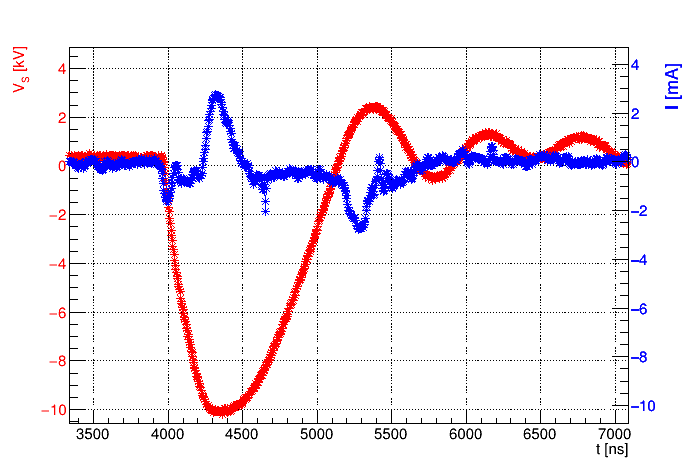
\includegraphics[width=0.6\textwidth]{Images/Electric/tenscurr_f5_t8.png}
 \caption{Example measure with source B for $f = \SI{5}{\kilo\hertz}$ and $\Delta t = \SI{8}{\micro\second}$}
 \label{fig:tens_curr}
\end{figure}


Data analysis is done as before, cleaning measures from noise, estimating the peak and it's error. Results are shown in figures \ref{fig:Vpp_gas} and \ref{fig:I_gas}, measures where the current peak is not distinguishable are excluded from plots.
\begin{figure}
 \centering
 \subfloat[Source A]{
    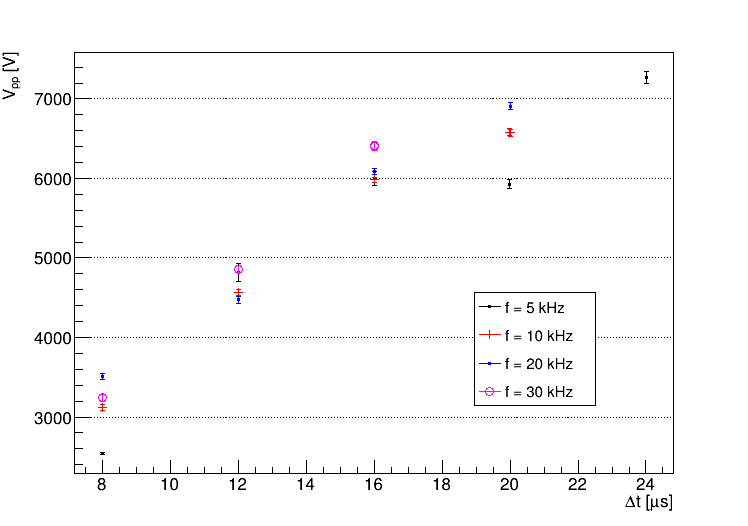
\includegraphics[width=0.6\textwidth]{Images/Electric/Vpp_gas_A.png}
 }
 
 \subfloat[Source B]{
    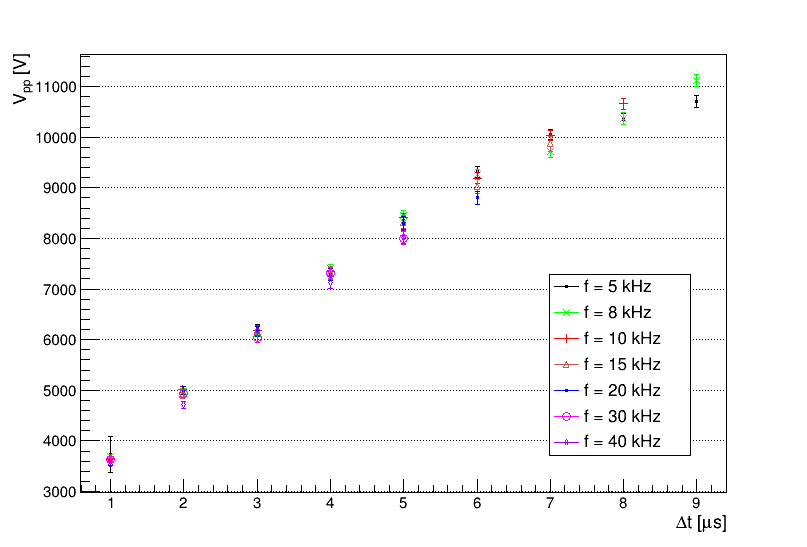
\includegraphics[width=0.6\textwidth]{Images/Electric/Vpp_gas_B.png}
 }
 \caption{Absolute peak's values of secondary circuit output in function of $\Delta t$ at different $f$, with an helium flux of $\SI{2}{\liter/\minute}$, for both sources.}
 \label{fig:Vpp_gas}
\end{figure}

\begin{figure}
 \centering
 \subfloat[Source A]{
    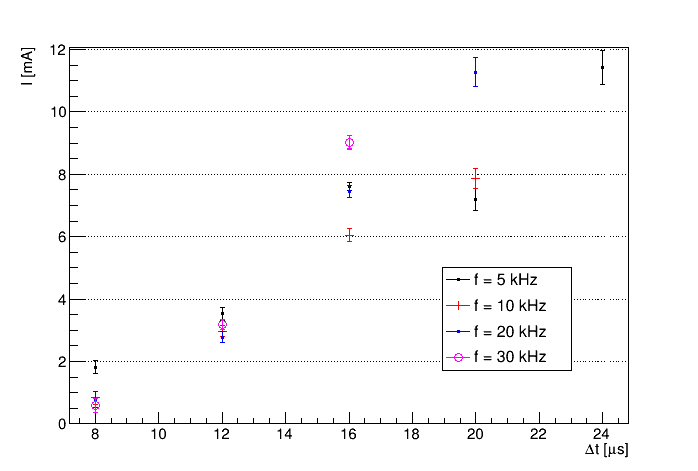
\includegraphics[width=0.6\textwidth]{Images/Electric/I_gas_A.png}
 }
 
 \subfloat[Source B]{
    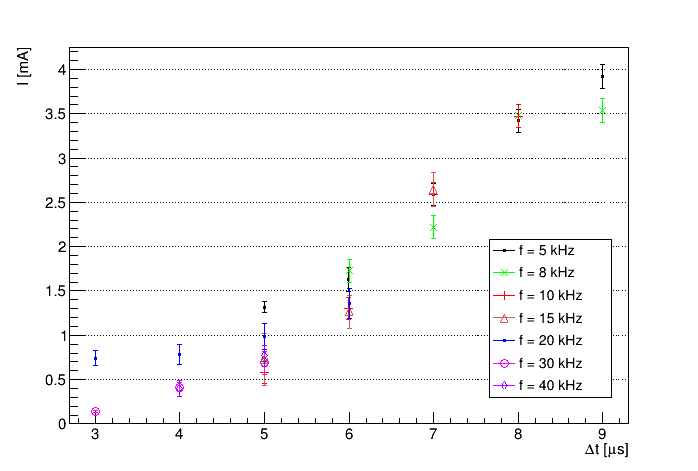
\includegraphics[width=0.6\textwidth]{Images/Electric/I_gas_B.png}
 }
 \caption{Absolute peak's value of current intensity on copper target with an helium flux of $\SI{2}{\liter/\minute}$, in function of $\Delta t$ at different $f$, for both sources.}
 \label{fig:I_gas}
\end{figure}

Tension peaks are slightly lower then values without gas, as expected seeing the plume as an additional load at the end of the circuit (\cite{lieberman1994principles}), but the linear behavior for $V_{pp} \le \SI{10}{\kilo\volt}$ remains and we can compare linearity for different frequencies. Current intensities grows with tension and are higher for source A, as expected given different distances electrode-target. Analysis of linearity also for those measures can show if there is a different behavior changing pulse frequency or source.
Figures \ref{fig:lingas_Vpp} and \ref{fig:lingas_I} shows results of the linearity study at different frequencies.
Tension values, for both sources, are scattered around the mean value parameter without a clear behavior, confirming independence hypotesis of voltage growth from pulses frequencies. For source A we find a slope parameter $m_{V} = \SI{0.366(1)}{\kilo\volt/\micro\second}$, for source B $m_{V} = \SI{1.145(8)}{\kilo\volt/\micro\second}$, larger due to the different circuit, as mentioned before.
Current values shows a different behavior: in source A we find a stady increase of parameters with higher frequencies, in source B data are more scattered and we couldn't extrapolate a behavior. However current slope is in the same range of values for the sources, with a maximum for source A of $m_{I} = \SI{1.10(1)}{\milli\ampere/\micro\second}$ and for source B of $m_{I} = \SI{1.04(17)}{\milli\ampere/\micro\second}$.
An explanation for parameter's trend in source A it's that for higher frequencies the interval between two pulses it's smaller and oscillations of electrode potential after a pulse influences more gas ionized fraction, so mean density value of charged particles is higher for higher frequencies. 
Due to low signal to noise ratio in measures for source B, it is not possible to esclude a relation between current slope (how much current intensity grows increasing opening time) and pulse frequency, however it is established a maximum limit value to take into consideration when using the device.

\begin{figure}
 \centering
 \subfloat[Source A]{
    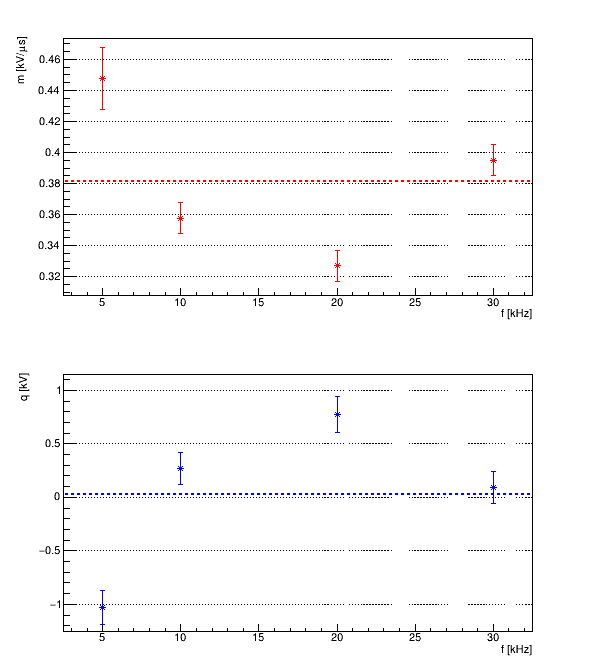
\includegraphics[width=0.4\textwidth]{Images/Electric/mq_V_gas_A.png}
 }
 \subfloat[Source B]{
    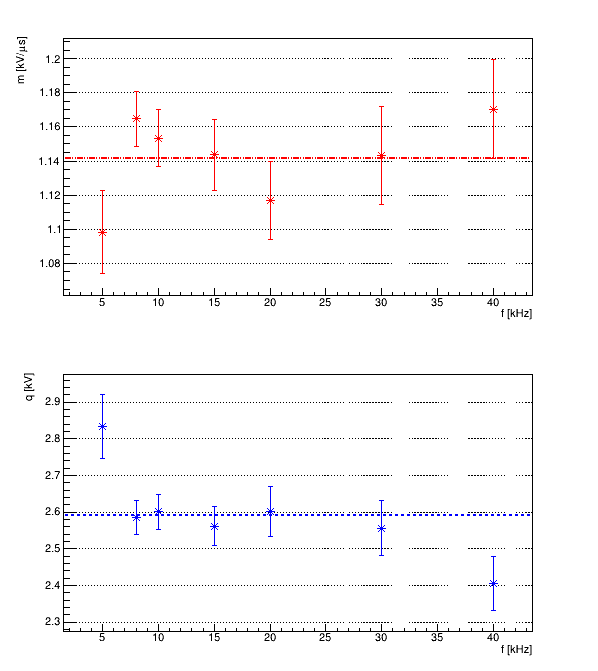
\includegraphics[width=0.4\textwidth]{Images/Electric/mq_V_gas_B.png}
 }
 \caption{Voltage peaks are fitted with a linear function $V_{peak} = m \Delta t + q$, in figure we see fit parameters at different frequencies for both sources, in dashes the mean value.}
 \label{fig:lingas_Vpp}
\end{figure}


\begin{figure}
 \centering
 \subfloat[Source A]{
    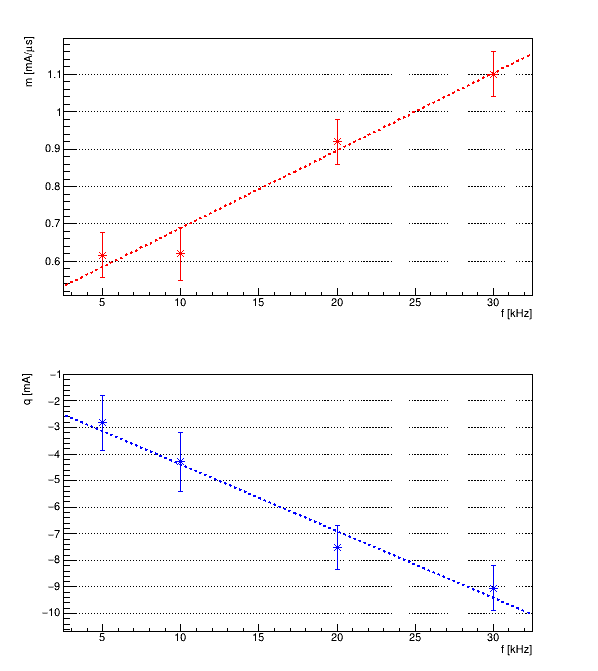
\includegraphics[width=0.4\textwidth]{Images/Electric/mq_I_gas_A.png}
 }
 \subfloat[Source B]{
    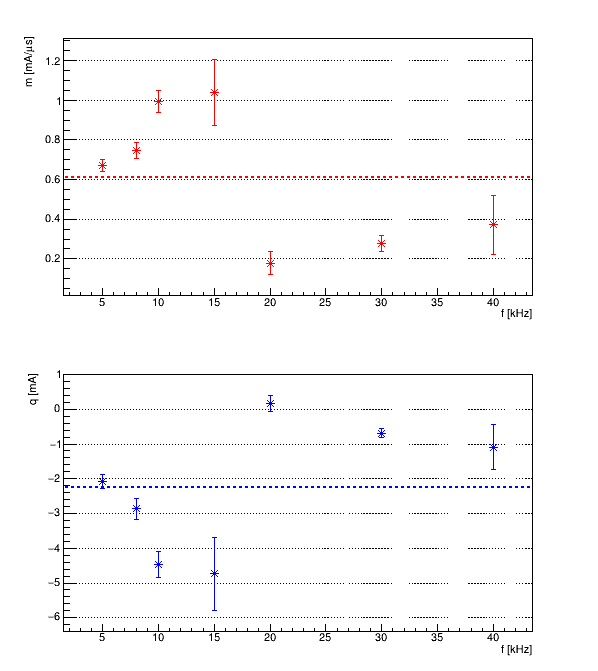
\includegraphics[width=0.4\textwidth]{Images/Electric/mq_I_gas_B.png}
 }
 \caption{Current peaks are fitted with a linear function $I_{peak} = m \Delta t + q$, in figure we see fit parameters at different frequencies for both sources. For source A we see in dashes a linear fit, for source B the mean value.}
 \label{fig:lingas_I}
\end{figure}


\subsection{Plasma impedance}
From tension and current measuraments we can define plasma's electric behavior, in this subsection source B measures are used to estimate plasma impedance. Tension output from head's transformer can be modelized as a dumped sine wave around the peak, as in equation \ref{eq:dmpsin}.
\begin{equation}
 V_{S} = V_{0} + V_{\text{pulse}} \sin{(2 \pi f_{V_{s}} t)} e^{-t/\tau}
 \label{eq:dmpsin}
\end{equation}

This formula gives an explicit parametrization for $f_{V_{s}}$ that is an estimation of the frequency of the single pulse (the frequency that defines rise and fall of the pulse, different from the work frequency of different pulses imposed by Arduino, called $f$). This parameter is important because plasma's electric behavior depends on this frequency, analyzing signal with different frequencies $f_{V_{s}}$ it's possible to understand plasma's parameters. Frequency pulse it's different for every opening time of the circuit, $\Delta t$, but it's constant when changing frequency of pulses, as explained before analyzing tension outputs at different frequencies. In figure \ref{fig:fitexp} are presented examples of a peak fitted with the function in formula \ref{eq:dmpsin} and it's fourier transform to show peak frequency corresponding to $f_{V_s}$ for that specific $\Delta t$. In figure \ref{fig:parexp} are shown different resulting parameters for different $\Delta t$.

\begin{figure}
 \centering
 \subfloat[Dumped sin fit]{
    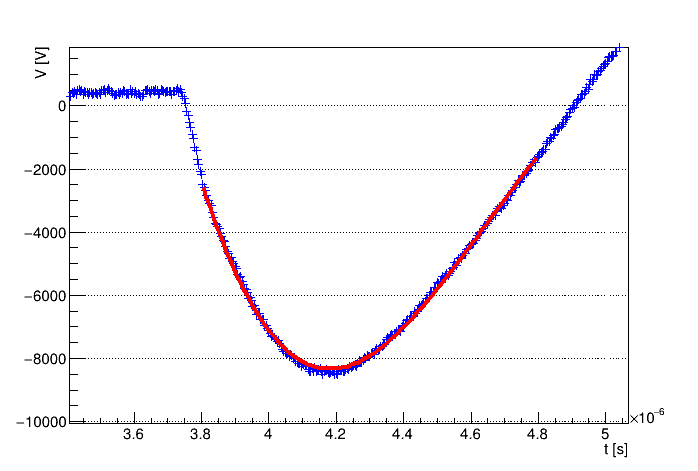
\includegraphics[width=0.4\textwidth]{Images/Electric/VFitexp_f8_t5.png}
 }
 \subfloat[Fourier transform]{
    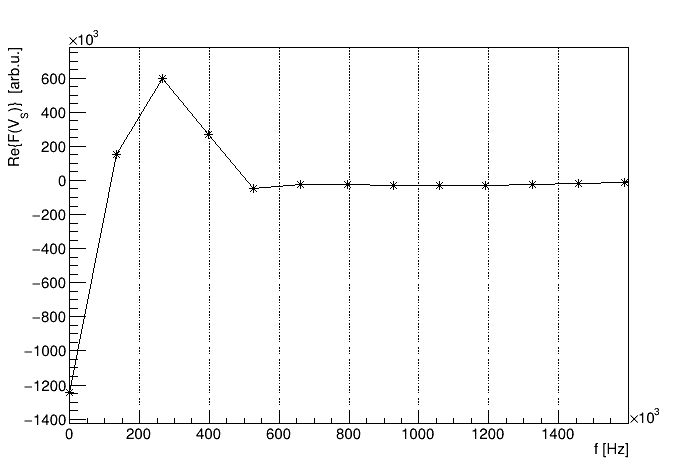
\includegraphics[width=0.4\textwidth]{Images/Electric/Trasf_f8_t5_clean.png}
 }
 \caption{On the left example fit of a tension peak, $f = \SI{8}{\kilo\hertz}$ $\Delta t = \SI{5}{\micro\second}$ with function \ref{eq:dmpsin}; on the right the fourier transform of the measure in the interval [$3-\SI{6}{\micro\second}$] that shows the frequency peak $f_{V_s}$}
 \label{fig:fitexp}
\end{figure}

\begin{figure}
 \centering
 \subfloat[$V_{\text{pulse}}$]{
    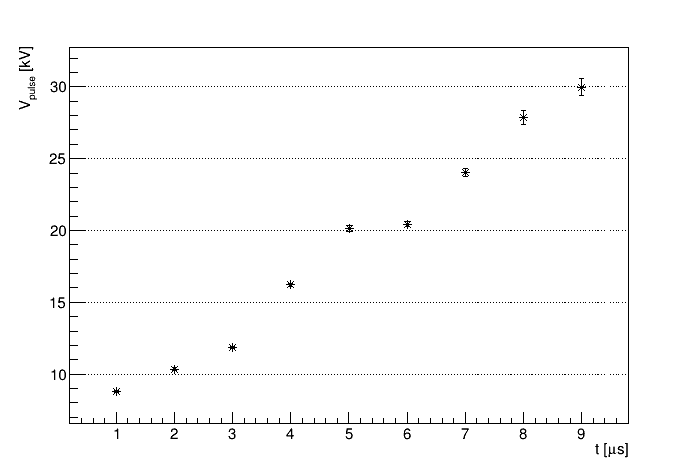
\includegraphics[width=0.4\textwidth]{Images/Electric/fitexp_V0_f8.png}
 }
 
 \subfloat[$\tau$]{
    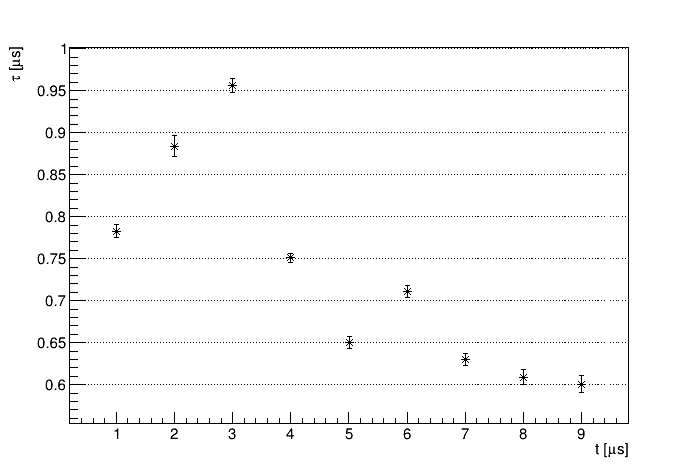
\includegraphics[width=0.4\textwidth]{Images/Electric/fitexp_tau_f8.png}
 }
 \subfloat[$f_{V_s}$]{
    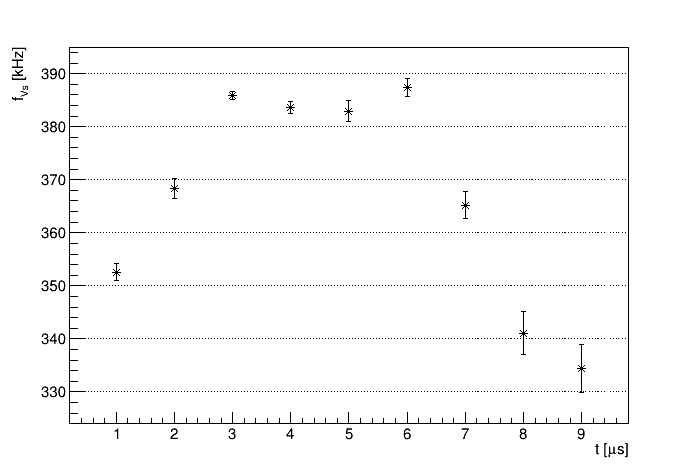
\includegraphics[width=0.4\textwidth]{Images/Electric/fitexp_w_f8.png}
 }
 \caption{Fit parameters of pulses with $f=\SI{8}{\kilo\hertz}$ for different $\Delta t$.}
 \label{fig:parexp}
\end{figure}

Fit parameters follows always those presented: as expected, with higher opening times $ V_{\text{pulse}} $ grows while $f_{V_{s}}$ and $\tau$ have their own behaviors that depends from tension secondary output $V_s$.
To estimate plasma's impedance it's useful to observe that voltage peak is quite large in time: it varies of less then $3\%$ of peak's value in an interval of $\SI{150}{\nano\second}$ around it. As tension and current peaks times differs always by a time interval $|t_{V_p} - t_{I_p}| \leq \SI{150}{\nano\second}$, it's possible to assume $V_{t_{I_p}} \simeq V(t_{V_p})$, i.e. that tension during the current peak maximum is equal to tension's peak value. With this approximation, it makes sense to plot tension's peak values against current's peak values, as in figure \ref{fig:viplot}, and given a $\Delta t$ it's possible to give an estimation of impedance module as $Z = \frac{V_{p}}{I_{p}}$. Resulting impedance are shown in figure \ref{fig:zest}, changing opening times and changing frequency of single pulse $f_{V_{s}}$.

\begin{figure}
 \centering
 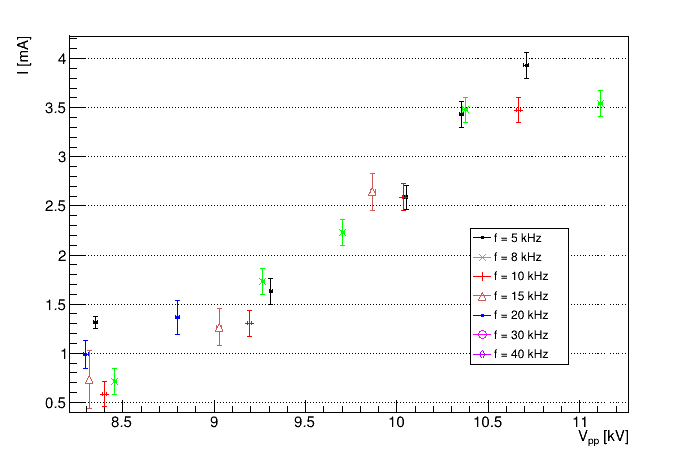
\includegraphics[width=0.6\textwidth]{Images/Electric/VI_B.png}
 \caption{Tension's peak values against current's peak values for different $\Delta t$ and frequencies.}
 \label{fig:viplot}
\end{figure}

\begin{figure}
 \centering
 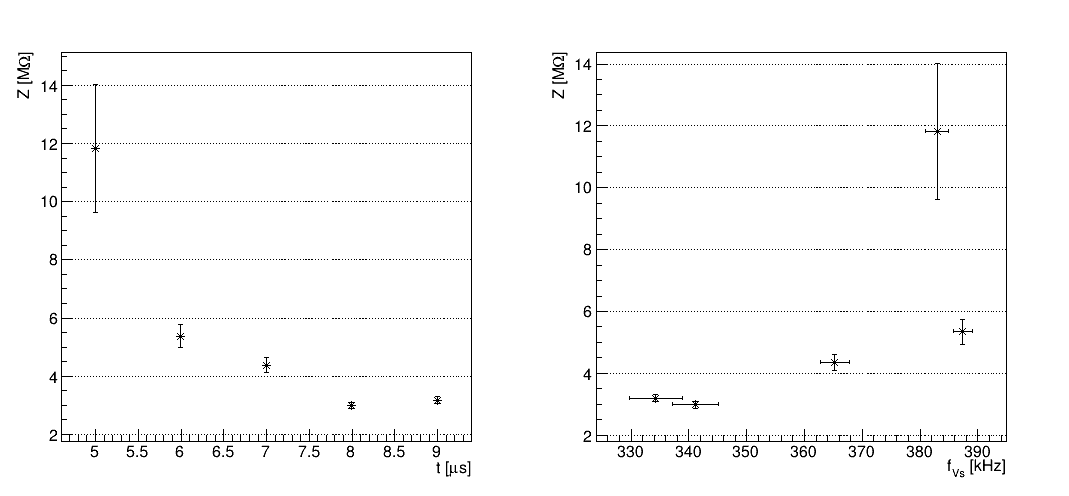
\includegraphics[width=0.8\textwidth]{Images/Electric/z_f8.png}
 \caption{Impedance module estimation for different opening times (left) corresponding to different frequencies (right).}
 \label{fig:zest}
\end{figure}

From the graphs it's possible to extrapolate that plasma impedance goes from $\SI{2.98(11)}{\mega\ohm}$ to $\SI{11.82(219)}{\mega\ohm}$, with near constant values in the range of opening times $7-\SI{9}{\micro\second}$.
From a deeper analysis and specific measures it could be possible to expand the analysis here presented and estimate plasma's electrical resistance, capacitance or induttance.

\subsection{Effective current}
Current effects in applications on biological tissues have to take into consideration current intensity in a time interval tipically larger then the pulse widths used in our sources (\cite{doi:10.1002/ppap.200731208}, \cite{unipd:ceciliaDBD}). It's possible to estimate an effective current that is more appropriate to take into consideration when evaluating damage due to currents, as a mean of current intensity in a defined time interval calculated with equation \ref{eq:ieff}, taking $t_2-t_1 = \SI{1}{\milli\second}$. The effective current takes into consideration that current values are very small for all the time between two pulses.
\begin{equation}
 \centering
 I_{\text{eff}} = \frac{1}{(t_2-t_1)}\sqrt{\int_{t_1}^{t_2} I^2 \,dt}
 \label{eq:ieff}
\end{equation}

Figure \ref{fig:ieff} shows effective currents measured for both sources. Values are significantly smaller then maximum peak values, expecially for source B where oscillations after the main peak are smaller. The maximum value for the two sources is given by $I_{\text{eff} A} = \SI{2.47(7)}{\milli\ampere}$ and $I_{\text{eff} B} = \SI{0.23(1)}{\milli\ampere}$.

\begin{figure}
 \centering
 \subfloat[Source A]{
    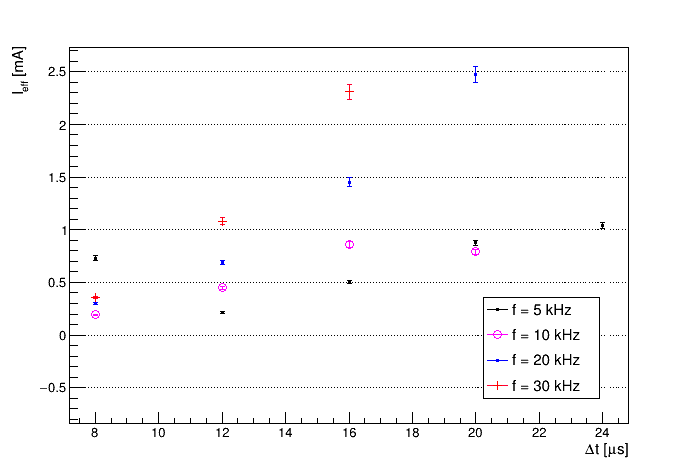
\includegraphics[width=0.4\textwidth]{Images/Electric/Ieff_A.png}
 }
 \subfloat[Source B]{
    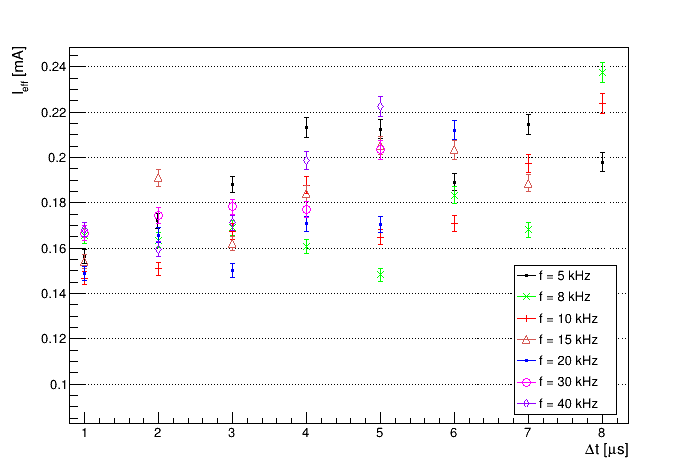
\includegraphics[width=0.4\textwidth]{Images/Electric/Ieff_B.png}
 }
 \caption{Effective currents in a time interval of $\SI{1}{\milli\second}$.}
 \label{fig:ieff}
\end{figure}


\subsection{Time intervals}
Time width of signal affects reaction's probabilities (chapter \ref{ch:shape}) and plasma's power deposition(chapter \ref{ch:temperature}), here we try to give an estimate of those time intervals. It can be defined as the FWHM of measured peaks, evaluated as the time when we measure half of tension or current maximum value. As the characterization of the sources shows an almost equal behavior, this study is made only for the latest version of the source, that's the only one used in the following chapters. Results are shown in figure \ref{fig:times}.
For every frequence there is a quadratic behavior of tension widths with a minimum for a $\Delta t = \SI{5}{\micro\second}$ that depends on circuit scheme. It is possible to give an estimation of pulse width with a mean value between this minimum and maximum values obtained for $\Delta t = \SI{1}{\micro\second}$, it is $T_{V} = \SI{963(15)}{\nano\second}$. For currents, widths have great uncertainity where the peak is low, but it is possible to evaluate a mean value for $\Delta t \ge \SI{6}{\micro\second}$, and it is $T_{I} = \SI{968(28)}{\nano\second}$.
Values from the two measures are compatible and they are a good estimation of pulse time duration.

\begin{figure}
 \centering
 \subfloat[Voltage]{
    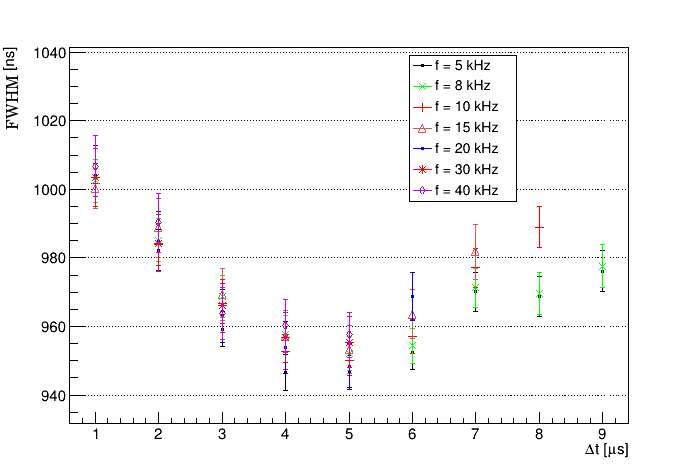
\includegraphics[width=0.4\textwidth]{Images/Electric/tempi_V.png}
 }
 \subfloat[Current]{
    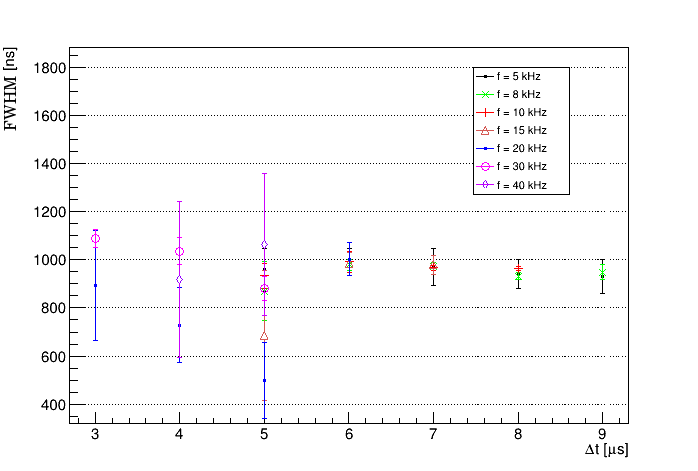
\includegraphics[width=0.4\textwidth]{Images/Electric/tempi_I.png}
 }
 \caption{FWHM of tension and current peaks varying opening time, for different frequencies.}
 \label{fig:times}
\end{figure}


\begin{comment}

\subsection{Corrente efficace}
Durante l'applicazione del plasma su tessuti vivi bisogna considerare il tempo di reazione effettivo del bersaglio, l'impulso di corrente alle frequenze di lavoro della sorgente presenta un periodo inferiore rispetto questi tempi. Per valutare gli effetti del trattamento viene calcolato il valore della corrente efficace che fluisce sulla piastra bersaglio in un tempo di \SI{1}{\milli\second}, dell'ordine di grandezza dei tempi di risposta da considerare (vedi articolo?), utilizzando la formula in \ref{eq:ieff}.
\begin{equation}
 \centering
 I_{\text{eff}} = \frac{1}{(t_2-t_1)}\sqrt{\int_{t_1}^{t_2} I^2 \,dt}
 \label{eq:ieff}
\end{equation}

In Figura \ref{fig:correff} vengono presentati i valori della corrente efficace in maniera simile a quanto fatto per le misure di corrente precedentemente.
A parità di tempo di apertura del circuito, una maggiore frequenza implica che nel tempo scelto di \SI{1}{\milli\second} vi sarà un numero di periodi maggiore, aumentando la corrente efficace nel circuito. In figura si vede come mediamente la corrente efficace sia più grande a frequenze maggiori, ma assume sempre valori inferiori ai \SI{3}{\milli\ampere}.

\begin{figure}
\centering
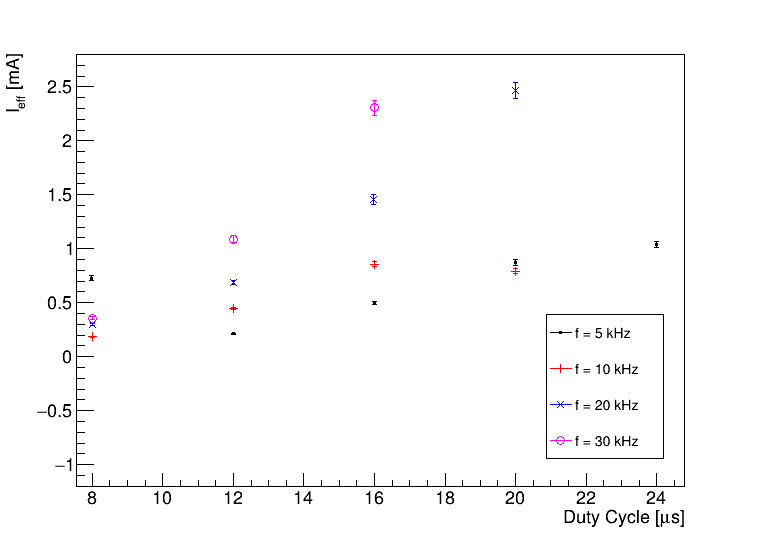
\includegraphics[width=.7\textwidth]{Immagini/ieff.png}
\caption{Corrente efficace calcolata al variare del tempo di apertura del circuito e per diverse frequenze.}
\label{fig:correff}
\end{figure}

\end{comment}


\begin{comment}
La sorgente di plasma funziona tramite l'applicazione di un'alta differenza di potenziale tra gli elettrodi separati da materiale dielettrico, come descritti nel capitolo \ref{ch:sorgente}. La tensione in ingresso nel circuito  della testa della sorgente vengono amplificati fino a tensioni di alcuni \si{\kilo\volt}. Dall'arduino di controllo è possibile regolare il tempo di apertura del circuito in un range di [$2$-$20$] \si{\micro\second} e la frequenza di lavoro in un range di [$2$-$60$] \si{\kilo\hertz}. I parametri importanti per caratterizzare il funzionamento della sorgente saranno quindi tensione e corrente all'uscita del circuito secondario del trasformatore, al variare dei parametri di funzionamento. Utilizzando una lastra metallica posta a potenziale, è possibile misurare la corrente in un dato range temporale. È inoltre possibile stimare la corrente efficace che attraversa il bersaglio, importante nel valutare gli effetti dell'applicazione del plasma.

\section{Setup delle misure di tensione e corrente}
Si vogliono effettuare misure di tensione della sorgente sia senza immissione di elio, senza formazione della plume di plasma, sia nelle condizioni di funzionamento tipiche, con flusso di elio di $\SI{2}{\liter/\minute}$.
Le tensioni vengono misurate tramite una sonda \emph{...} con attenuazione $\times1000$, le correnti tramite una sonda \emph{Tektronix CT2} che per una corrente di \SI{1}{\milli\ampere} restituisce un segnale di \SI{1}{\milli\volt}. I dati vengono letti su un oscilloscopio \emph{Yokogawa DL9040}, che permette il salvataggio dell'intera forma d'onda misurata nei diversi canali. 
Viene effettuata la caratterizzazione elettrica di entrambi i prototipi di sorgente, per i quali il circuito utilizzato è lo stesso, quindi non si aspettano variazioni significative.
\end{comment}



\begin{comment}

\subsection{Misure senza elio}
La sonda ad alta tensione viene collegata all'uscita del circuito secondario, mentre una sonda con attenuazione $\times10$ viene utilizzata per controllare il segnale in ingresso.
La sorgente viene azionata variando la frequenza ($f$) e duty cycle ($\Delta t$). Scelta la frequenza di lavoro, viene variata la duty cycle in un range utile, considerando il tempo necessario al terminare delle oscillazioni del segnale prima dell'arrivo di una nuova onda quadra (per frequenze maggiori si potrà arrivare a duty cycle minori).
Si ottengono curve come in figura \ref{fig:tensione_es}. La risoluzione della misura viene variata in modo da avere l'errore di misura minore possibile.

\begin{figure}
\centering
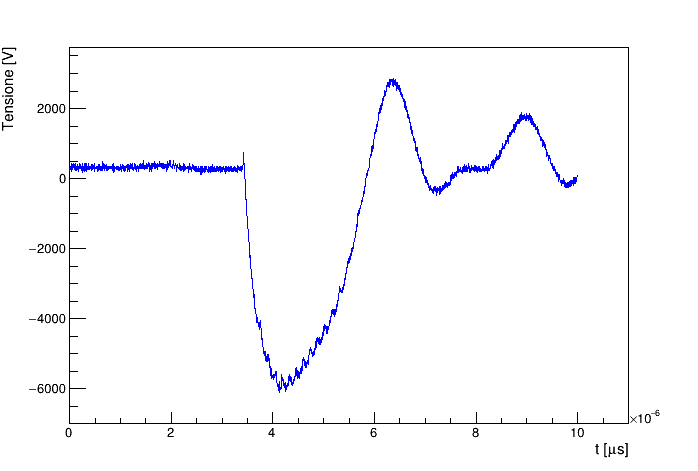
\includegraphics[width=.7\textwidth]{Immagini/tensione_es_2.png}
\caption{Esempio di misura di tensione, $f = \SI{5}{\kilo\hertz}$ e $\Delta t = \SI{16}{\micro\second}$, prototipo 1.}
\label{fig:tensione_es}
\end{figure}



\section{Presentazione misure ed analisi}
Sia per le misure di tensione che per le misure di corrente si trova un picco negativo come presentato nelle Figure \ref{fig:tensione_es} e \ref{fig:corrente_es}. Il picco di tensione ha valori tipici tra i $\num{3}$ e i $\SI{10}{\kilo\volt}$ in assenza o in presenza di gas, mentre quello di corrente tra i $\num{2}$ e i $\SI{12}{\milli\ampere}$.
L'analisi dei dati prevede la ricerca del massimo della tensione e della corrente nelle diverse configurazioni.

\subsection{Tensione di picco senza elio}
L'andamento medio delle misure presenta un picco negativo pronunciato, compatibile con i tempi di apertura del circuito. Dato un set, il valore di picco viene cercato calcolando la trasformata di Fourier del segnale (tramite le routine fftw3 delle librerie ROOT), tagliando le oscillazioni ad alta frequenza e ricostruendone una media. Nel segnale medio così ricostruito il valore del minimo viene trovato interpolando con una funzione di Landau attorno il minimo, in modo da riprodurre l'asimmetria del picco.
A queste misure viene aggiunto l'errore dovuto al taglio delle alte frequenze, preso come una media del valore assoluto dell'oscillazione del segnale tagliato. Viene inoltre aggiunto l'errore caratteristico dello strumento di misura, trascurabile rispetto l'errore dovuto alle oscillazioni veloci.
In figura \ref{fig:landau} un esempio del fit.

\begin{figure}
\centering
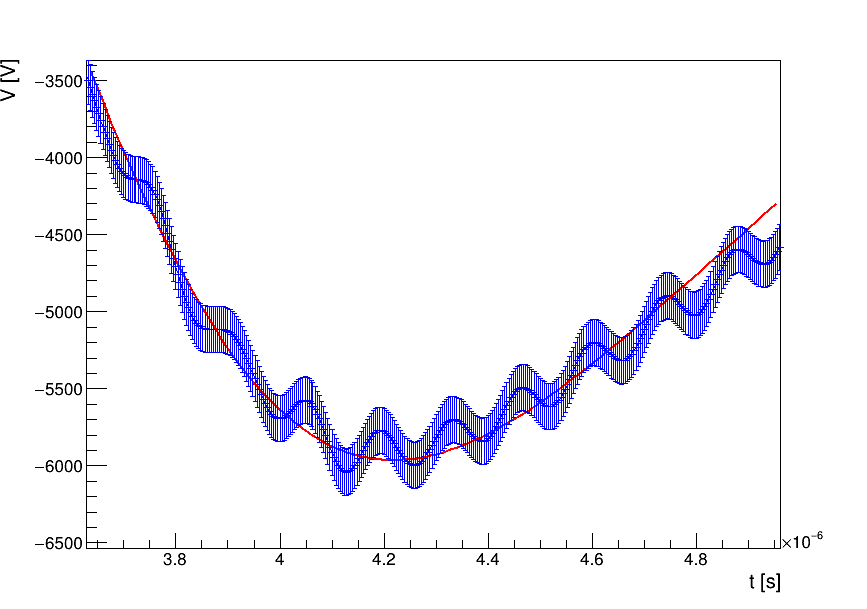
\includegraphics[width=.6\textwidth]{Immagini/esfiterr.png}
\caption{Esempio di fit del picco di tensione, $f = \SI{5}{\kilo\hertz}$ e $\Delta t = \SI{16}{\micro\second}$}
\label{fig:landau}
\end{figure}


Le tensioni del picco così calcolate, al variare della duty cycle per le diverse frequenze, sono presentate in figura \ref{fig:tensioni}.
Per tutte le frequenze di lavoro tra i $\SI{4}{\micro\second}$ e i $\SI{16}{\micro\second}$ risulta un andamento lineare, con tensione variabile tra i $\SI{2}{\kilo\volt}$ e i $\SI{9}{\kilo\volt}$. Aumentando ancora il tempo di apertura del circuito la tensione arriva a valori più elevati, fino un massimo di circa $\SI{10}{\kilo\volt}$, ma viene perso l'andamento lineare.


 \begin{figure}
\centering
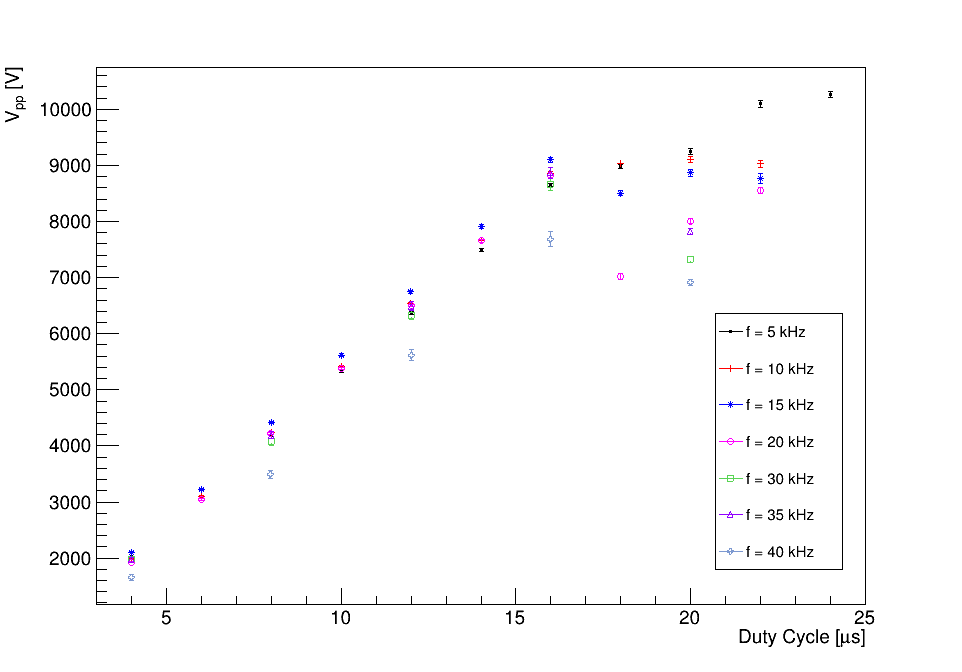
\includegraphics[width=.6\textwidth]{Immagini/nogas.png}
\caption{Tensioni al variare del tempo di apertura del circuito e per diverse frequenze.}
\label{fig:tensioni}
\end{figure}


Le misure non sembrano presentare un andamento in funzione della frequenza, per verificarlo vengono calcolati i coefficenti dell'interpolazione lineare per le varie frequenze, presentati in figura \ref{fig:fitlin}.
Viene confermata l'assenza di un andamento specifico al variare della frequenza.

\begin{figure}
\centering
\subfloat[][Pendenza delle rette.]
  {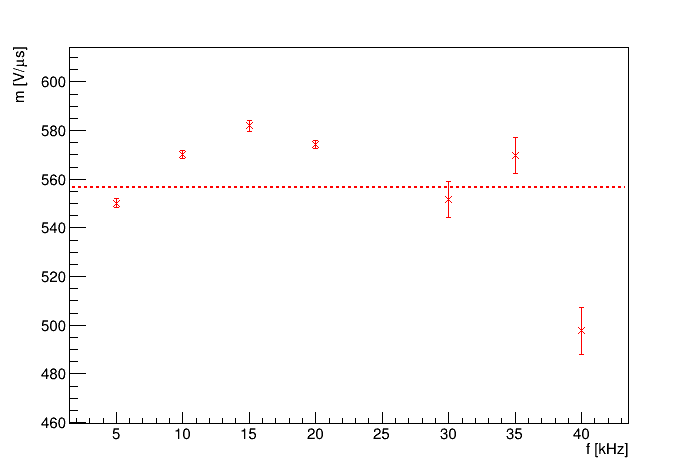
\includegraphics[width=.48\textwidth]{Immagini/m_freq_nogas.png}}
\subfloat[][Intercetta delle rette.]
  {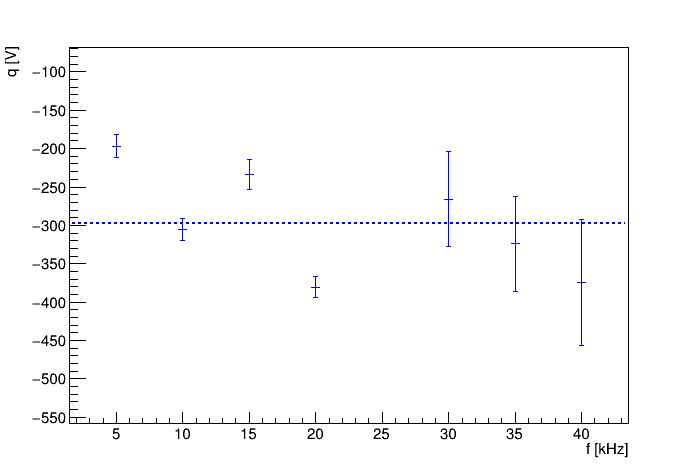
\includegraphics[width=.48\textwidth]{Immagini/q_freq_nogas.png}}
\caption{Parametri dell'interpolazione lineare dei set di misure senza immissione di gas(nel range $\Delta t$ stabilito), al variare della frequenza.}
\label{fig:fitlin}
\end{figure}

\end{comment}


\begin{comment}
\subsection{Misure con elio}
Per caratterizzare il funzionamento della sorgente nelle possibili condizioni di trattamento, vengono misurate contemporaneamente, su due diversi canali dell'oscilloscopio, tensione alla quale si trova l'elettrodo e corrente che fluisce nel plasma. Per la misura di corrente viene fatto impattare il plasma su una piastra di rame  di dimensioni \SI{2}{\centi\metre} $\times$ \SI{2}{\centi\metre} $\times$ \SI{0.5}{\centi\metre}, ad una distanza di \SI{1}{\centi\metre} dall'elettrodo della sorgente, collegata alla sonda di corrente.
Nuovamente vengono effettuate misure al variare di frequenza ($f$) e duty cycle ($\Delta t$), con le stesse modalità delle misure di tensione.
Tutte le misure sono effettuate con flusso di gas He pari a $\SI{2}{\litre/\minute}$.
Si ottengono curve come in figura \ref{fig:corrente_es}.

\begin{figure}
\centering
 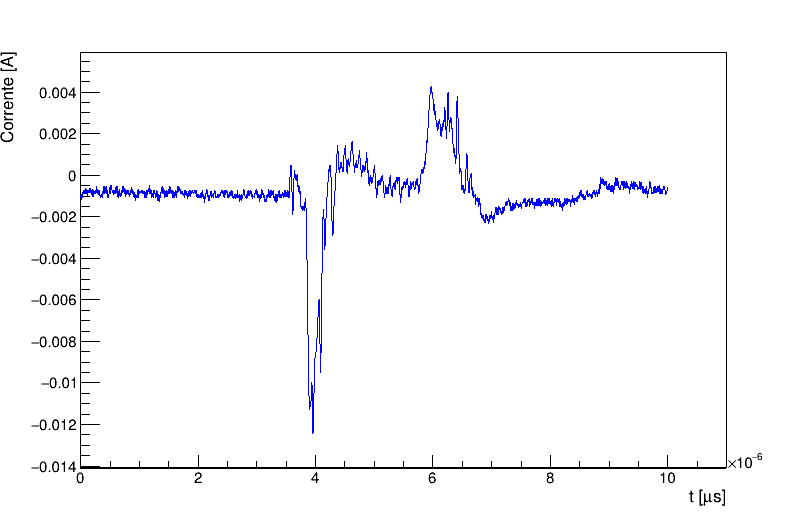
\includegraphics[width=.7\textwidth]{Immagini/corrente_es.png}
\caption{Esempio di misure di corrente per $f = \SI{5}{\kilo\hertz}$ e $\Delta t = \SI{24}{\micro\second}$, prototipo 1.}
\label{fig:corrente_es}
\end{figure}



\subsection{Tensione e corrente con elio}
Le misure di tensione presentano l'andamento trovato precedentemente, mentre le misure di corrente presentano un primo picco negativo seguito da un picco più basso di segno opposto, positivo. L'analisi proposta è uguale a quella pensata per i set di misure precedenti: vengono tagliate le oscillazioni ad alta frequenza, ricostruito il segnale (aggiungendo l'errore dovuto al taglio delle alte frequenze e agli strumenti di misura) e il valore del minimo viene trovato interpolando con una funzione di Landau. Da questo fit vengono calcolati valori e posizione del picco di tensione, del picco negativo di corrente e del picco positivo di corrente.
In figura \ref{fig:landau} un esempio del fit.

\begin{figure}
\centering
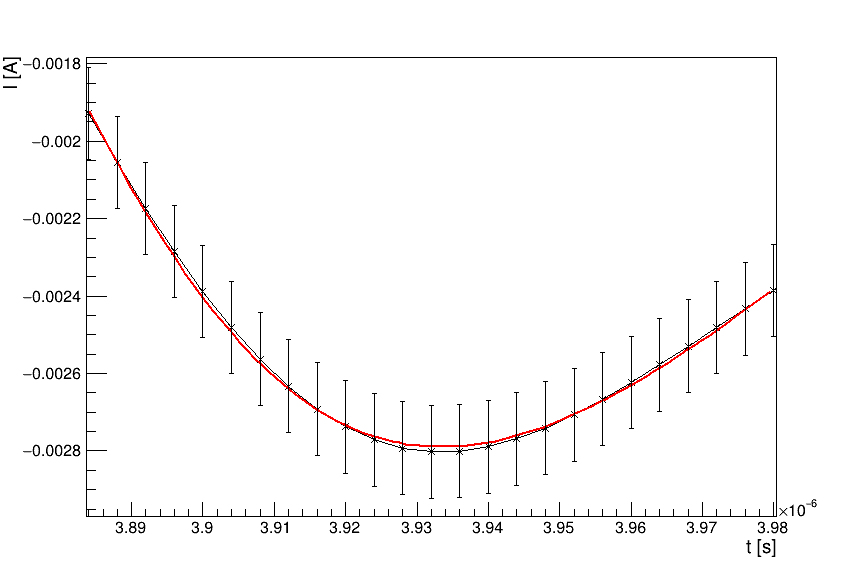
\includegraphics[width=.6\textwidth]{Immagini/es_fit_landau.png}
\caption{Esempio di fit del picco di corrente, $f = \SI{5}{\kilo\hertz}$ e $\Delta t = \SI{24}{\micro\second}$}
\label{fig:landau}
\end{figure}

Le tensioni del picco così calcolate, al variare della duty cycle per le diverse frequenze, sono presentate in figura \ref{fig:picchi}.
Nuovamente troviamo un andamento lineare per la tensione tra i $\num{4}$ e i $\SI{16}{\micro\second}$. Anche il picco negativo di corrente presenta questo andamento lineare, mentre per il picco positivo non è possibile identificare un comportamento simile, i valori si disperdono.

\begin{figure}
\centering
\subfloat[][Modulo del picco di tensione.]
  {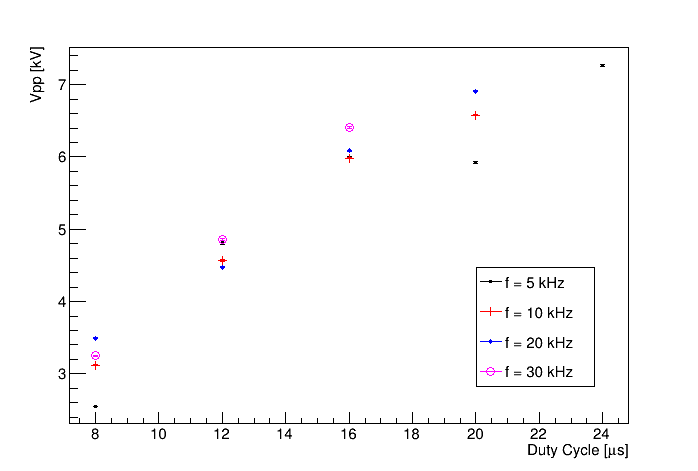
\includegraphics[width=.65\textwidth]{Immagini/vpp_corrente.png}}
\\
\subfloat[][Modulo del picco primario di corrente.]
  {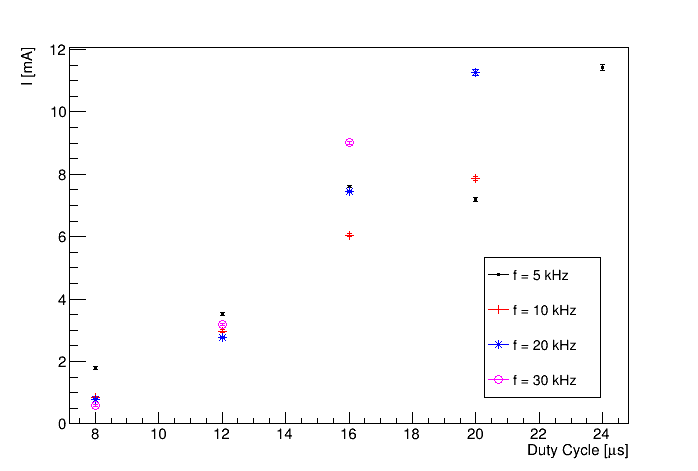
\includegraphics[width=.65\textwidth]{Immagini/I1_corrente.png}}
\\
\subfloat[][Picco secondario di corrente.]
  {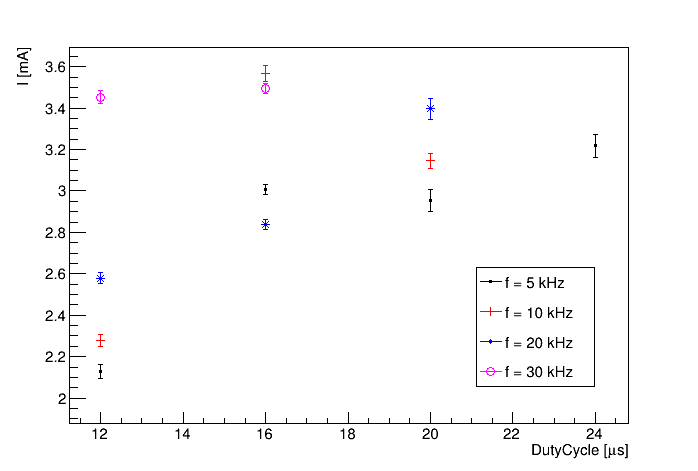
\includegraphics[width=.65\textwidth]{Immagini/I2_corrente.png}}
\caption{Valori dei picchi misurati al variare del tempo di apertura del circuito e per diverse frequenze.}
\label{fig:picchi}
\end{figure}


Nuovamente, per visualizzare in maniera esplicita l'effetto della variazione della frequenza, vengono calcolati i coefficenti dell'interpolazione lineare per le tensioni di picco e per le correnti di picco negativo, presentati in figura \ref{fig:fitlin_cor}. 
Per le tensioni risulta un comportamento identico al precedente, dove i valori si assestano attorno una media lievemente inferiore rispetto le misure in assenza di elio.
Per il valore massimo di corrente viene trovato un aumento in funzione della frequenza di funzionamento della sorgente.

\begin{figure}
\centering
\subfloat[][Pendenze dei picchi di tensione.]
  {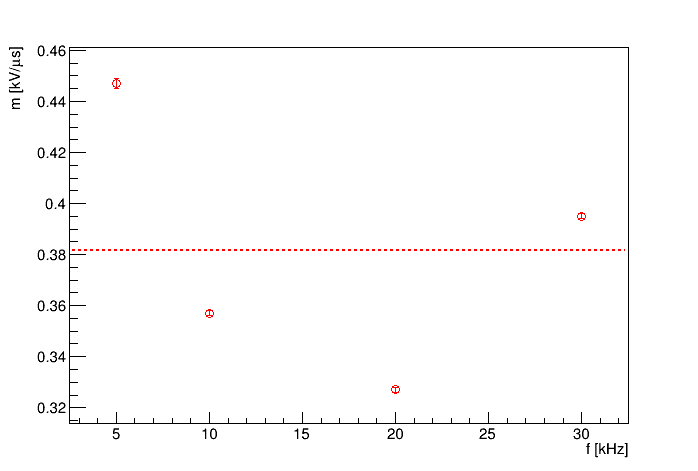
\includegraphics[width=.48\textwidth]{Immagini/mVpp_cor.png}}
\subfloat[][Intercette dei picchi di tensione.]
  {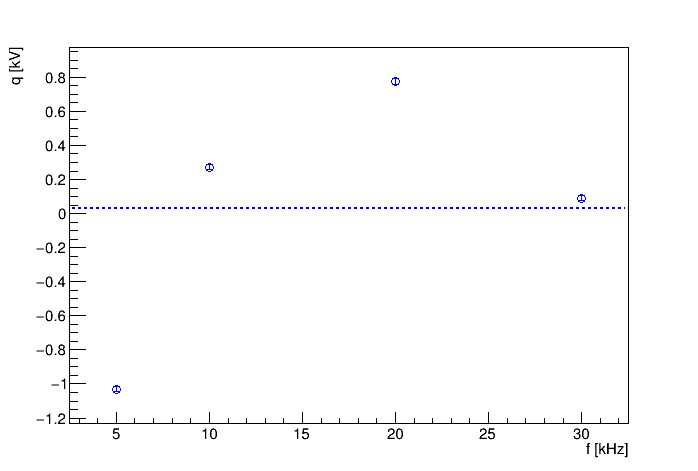
\includegraphics[width=.48\textwidth]{Immagini/qVpp_cor.png}}
\newline
\subfloat[][Pendenze dei picchi di corrente.]
  {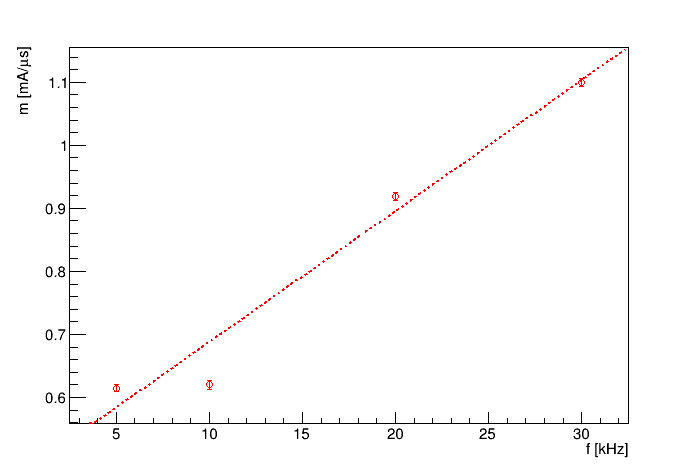
\includegraphics[width=.48\textwidth]{Immagini/mI1_cor.png}}
\subfloat[][Intercette dei picchi di corrente.]
  {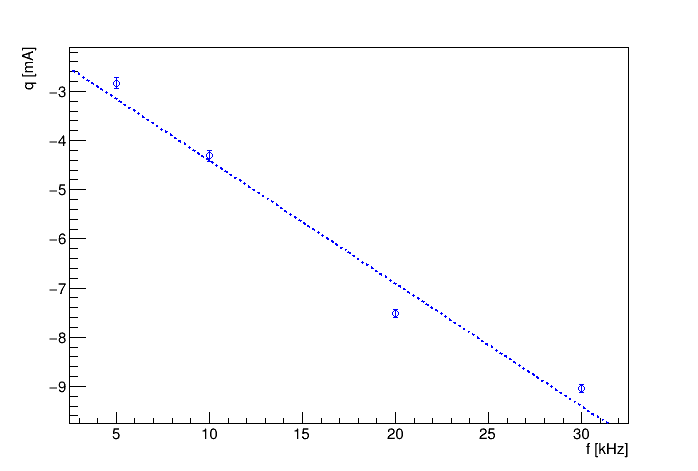
\includegraphics[width=.48\textwidth]{Immagini/qI1_cor.png}}
\caption{Parametri dell'interpolazione lineare dei picchi delle misure di tensione e corrente.}
\label{fig:fitlin_cor}
\end{figure}

\end{comment}



\begin{comment}

Data la possibilità di visualizzare contemporaneamente sia la tensione sia la corrente in uscita dal circuito, viene proposta un'analisi delle variazioni temporali tra i diversi picchi. In particolare viene calcolato il tempo tra i due picchi di corrente e tra il picco di tensione e il picco di corrente primario, mostrati in figura \ref{fig:tempi}.
In entrambi i casi non è possibile estrapolare un andamento particolare, indicando che non vi sono differenze significative nei tempi di salita dei picchi al variare del tempo di apertura del circuito e della frequenza.

\begin{figure}
\centering
\subfloat[][Tempo tra i picchi di corrente.]
  {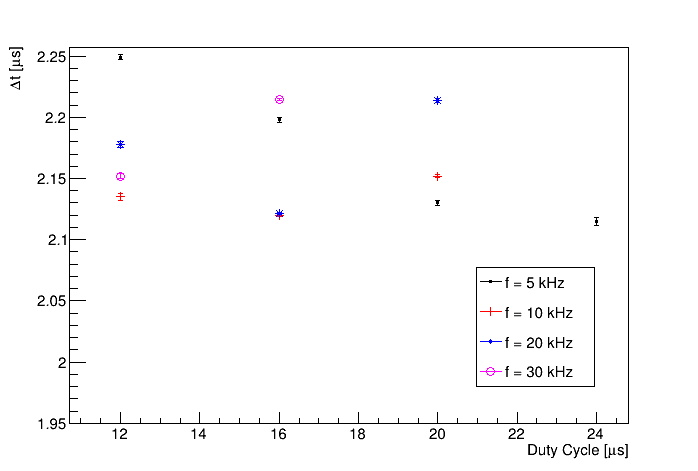
\includegraphics[width=.48\textwidth]{Immagini/ti2ti1.png}}
\subfloat[][Tempo tra picco tensione e primo picco di corrente.]
  {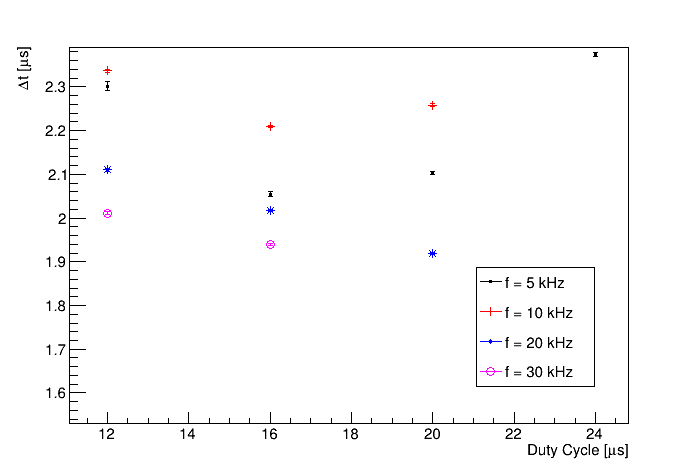
\includegraphics[width=.48\textwidth]{Immagini/ti1tv.png}}
\caption{Misura delle differenze temporali tra i picchi.}
\label{fig:tempi}
\end{figure}

\end{comment}

